% ============================================================
% Capítulo VIII — Aberración astronómica
% Traducción de "Théorie mathématique de la lumière" (1889), cap. VIII
% Original: §§231-243, páginas impresas 379-401
% Último capítulo del Volumen I; termina con las Conclusiones del volumen.
% ============================================================
\chapter{Aberración astronómica}
\label{cap:aberracion}

\noindent\textbf{231.} En el estudio de los diversos fenómenos ópticos que
hemos considerado hasta aquí, siempre hemos supuesto que el movimiento
vibratorio que da origen a la luz tenía lugar en un fluido particular, el
éter, repartido tanto en los medios materiales transparentes como en los
espacios interplanetarios. Es evidentemente imposible concebir la
propagación de la luz del Sol a la Tierra sin la existencia de un medio
elástico; en cambio, puede parecer superfluo y quizás poco filosófico
suponer la existencia del éter en los medios materiales. Sin embargo, el
fenómeno de la aberración astronómica, que pone en evidencia el movimiento
relativo del éter y del medio ponderable que este penetra, parece oponerse
absolutamente a la supresión de esta hipótesis; o, al menos, si se
rechazara esta hipótesis, la explicación de la aberración astronómica
tropezaría con dificultades tales que es preferible mantenerla. Digamos,
pues, algunas palabras sobre este fenómeno.

Se sabe que, cuando se apunta a un astro con un anteojo, el astro no se
encuentra sobre la recta que une el centro óptico del objetivo con el
punto de cruce de los hilos del retículo, es decir, sobre el eje óptico del
instrumento. No vemos, pues, un astro en su dirección real, y el ángulo de
esta dirección con el del eje óptico del anteojo se llama la \emph{aberración};
este desvío angular puede llegar hasta $20''$.

\section{Explicación de Bradley}

\noindent\textbf{232. Explicación de Bradley.} — La primera explicación
del fenómeno de la aberración se debe a Bradley; se apoya, por lo demás, en
la teoría de la emisión, que era entonces la adoptada. Sea $OA$
(figura~\ref{fig:cap8-1}) una recta que representa, en magnitud y
dirección, la velocidad de la que están animados los corpúsculos luminosos
emitidos por el astro. El observador, situado en la superficie de la
Tierra y arrastrado por el movimiento de esta, no podrá comprobar más que
la velocidad relativa del corpúsculo.

\begin{figure}[h]
\centering
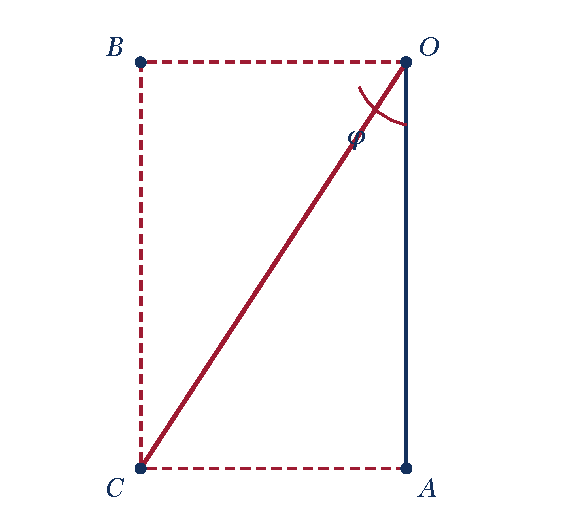
\includegraphics[width=0.7\textwidth]{figuras/pdf/cap08-fig1.pdf}
\caption{Composición de velocidades en la explicación de Bradley: $OA$
es la velocidad real de la luz, $OB$ la velocidad de arrastre del
observador (invertida), y $OC$ la diagonal que da la dirección
aparente.}
\label{fig:cap8-1}
\end{figure}

Esta velocidad relativa se obtendrá componiendo la velocidad real $OA$ con
la velocidad $OB$, igual y de signo contrario a la velocidad de arrastre
del observador; será, pues, $OC$. El observador verá el astro según la
dirección $CO$ en lugar de verlo en la dirección $AO$; por consiguiente, la
aberración será el ángulo $\varphi$. El valor de este ángulo será
evidentemente máximo cuando el cuadrilátero $OABC$ se vuelva rectángulo. En
este caso tendremos
\[
\tan\varphi = \frac{OB}{OA};
\]
o bien, siendo la velocidad $OA$ de la luz de unos $300\,000$ kilómetros
por segundo, y la velocidad de arrastre de un punto de la superficie de la
Tierra de solo $30$ kilómetros, tendremos aproximadamente
\[
\tan\varphi = \frac{30}{300\,000} = \frac{1}{10\,000}.
\]
El ángulo $\varphi$ correspondiente a este valor de la tangente es, como ya
hemos dicho, de unos $20$ segundos.

\begin{notahistorica}
James Bradley descubrió la aberración de la luz estelar en el curso de
observaciones realizadas entre 1725 y 1728, mientras intentaba medir la
paralaje de las estrellas, y comunicó su explicación a la Royal Society a
comienzos de 1729 (enero de 1728 según el calendario inglés de la época).
Fue la primera prueba observacional directa del movimiento de la Tierra
en el espacio —independiente de la paralaje, que no se mediría con éxito
hasta más de un siglo después— y permitió, de paso, una de las primeras
estimaciones precisas de la velocidad de la luz.
\end{notahistorica}

\section{Explicación ondulatoria}

\noindent\textbf{233. Explicación elemental en la teoría de las
ondulaciones.} — En la hipótesis de las ondulaciones, la explicación
elemental del fenómeno es igualmente simple. Sea $A$
(figura~\ref{fig:cap8-2}) el centro óptico del objetivo de un anteojo, $B$
el cruce de los hilos del retículo, y $AE$ la dirección de un rayo luminoso
proveniente de una estrella $E$. Si la Tierra estuviera inmóvil, los tres
puntos $E$, $A$ y $B$ estarían en línea recta; pero, a causa del movimiento
de la Tierra, el punto $B$ ha pasado a $B'$ durante el tiempo que el rayo
luminoso empleó en recorrer el camino $AB'$. El rayo luminoso que viene a
herir el ojo del observador tiene, pues, por dirección real $EAB'$,
mientras que su dirección aparente es la del eje óptico, es decir, la de
una paralela a $BA$ trazada por $B'$; la aberración es, por tanto, el
ángulo $BAB' = \varphi$. Si designamos por $V$ la velocidad de propagación
de las ondas luminosas en el éter inmóvil y por $v$ la velocidad de un
punto de la superficie de la Tierra, supuesta paralela a $BB'$, tendremos:
\[
\sin\varphi = \frac{BB'}{AB'} = \frac{vt}{Vt} = \frac{v}{V}.
\]

\begin{figure}[h]
\centering
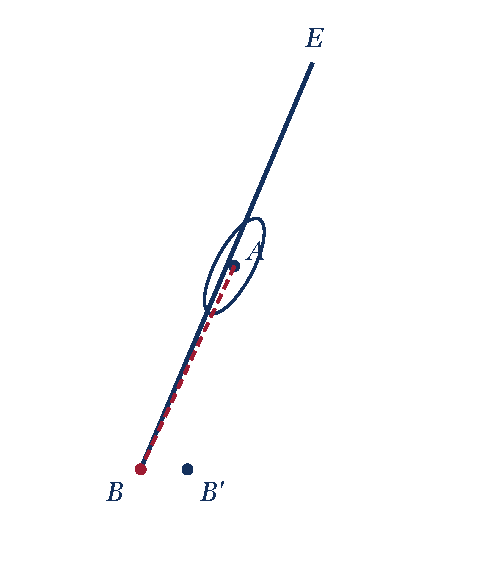
\includegraphics[width=0.55\textwidth]{figuras/pdf/cap08-fig2.pdf}
\caption{Explicación ondulatoria de la aberración: el rayo real $EAB'$
y la dirección aparente, paralela a $AB$ trazada por $B'$.}
\label{fig:cap8-2}
\end{figure}

Como el ángulo $\varphi$ es muy pequeño, se puede confundir el valor del
ángulo con el de su tangente o con el de su seno; por consiguiente,
volvemos a encontrar para el máximo de $\varphi$ el mismo valor que por la
explicación de Bradley.

Este razonamiento supone que el éter contenido en el anteojo está inmóvil
en el espacio, que no participa del movimiento de la Tierra. En efecto,
cuando un medio elástico se desplaza, las vibraciones que transmite
participan de ese movimiento; así, se sabe que la velocidad del sonido en
el aire en movimiento depende de la velocidad del aire, y la influencia del
viento sobre la velocidad de propagación del sonido es una prueba
evidente. Por consiguiente, si el éter contenido en el anteojo se
encontrara arrastrado con ella, la velocidad de propagación de la luz en el
tubo del anteojo sería la compuesta $V'$ de la velocidad $V$ y de la
velocidad de arrastre $v$ del medio elástico. Pero, por otra parte,
participando el observador del movimiento de la Tierra, la velocidad
relativa de la luz sería para él la resultante de $V'$ y de $-v$, es decir,
$V$. Los fenómenos observados serían entonces los mismos que si el éter y
el observador estuvieran inmóviles; por consiguiente, no habría
aberración, consecuencia contraria a la experiencia.

\section{El arrastre parcial del éter}

\noindent\textbf{234. El éter contenido en un medio material en movimiento
es parcialmente arrastrado.} — Pero, ¿está el éter inmóvil cuando atraviesa
un medio más refringente que el aire? Una experiencia de los astrónomos de
Greenwich nos permite responder que el éter es \emph{parcialmente} arrastrado
y que su velocidad de arrastre depende del índice de refracción de la
sustancia atravesada por la luz. En el aire mismo debería haber un arrastre
parcial del éter, muy débil es cierto puesto que el aire es poco
refringente; pero para que la explicación precedente fuera del todo
rigurosa, habríamos debido suponer que el tubo del anteojo estaba vacío de
aire.

La experiencia de los astrónomos de Greenwich consistía en apuntar una
estrella con un anteojo lleno de aire, y luego con el mismo anteojo cuyo
tubo estaba lleno de agua; comprobaron que, en ambos casos, la posición
aparente del astro era la misma. Analicemos esta experiencia y busquemos
sus consecuencias.

\begin{figure}[h]
\centering
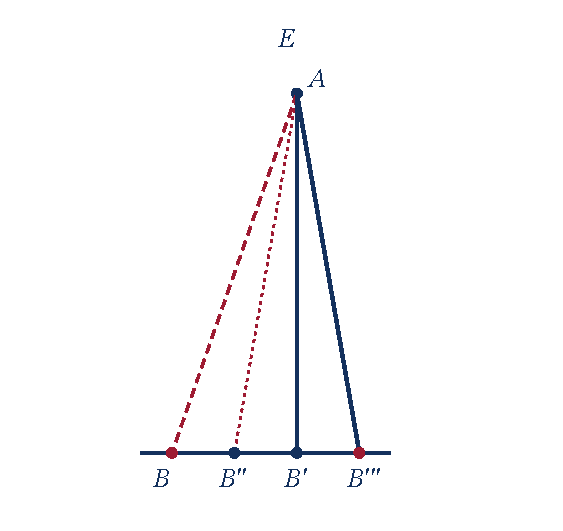
\includegraphics[width=0.7\textwidth]{figuras/pdf/cap08-fig3.pdf}
\caption{El experimento de los astrónomos de Greenwich: posiciones del
cruce de los hilos del retículo bajo las distintas hipótesis sobre el
arrastre del éter en el agua.}
\label{fig:cap8-3}
\end{figure}

Sea $EAB'$ (figura~\ref{fig:cap8-3}) la dirección de propagación de la luz
en el anteojo, que supondremos vacío de aire, en la hipótesis en que el
éter no participa del movimiento de la Tierra. Si admitimos que ocurre lo
mismo para el éter contenido en el agua en movimiento, el rayo $EC$,
penetrando oblicuamente en ese medio, se refractaría siguiendo $AB''$
acercándose a la normal. La imagen de la estrella se formaría en $B''$.
Ahora bien, propagándose la luz más lentamente en el agua que en el vacío,
el punto de cruce $B$ de los hilos del retículo del anteojo se encontrará,
a causa del movimiento de la Tierra, en un punto $B'''$, situado a la
derecha de $B'$, cuando las vibraciones luminosas lleguen al plano del
retículo. Estando los puntos $B''$ y $B'''$, el primero a la izquierda, el
segundo a la derecha de $B'$, no pueden coincidir, y por consiguiente la
imagen de la estrella ya no se encontraría en el punto de cruce de los
hilos del retículo. Debemos, pues, admitir, para estar de acuerdo con la
experiencia, que el éter que propaga la luz en el agua es arrastrado, al
menos parcialmente, por el movimiento de la Tierra.

Busquemos la velocidad de arrastre. Designando por $i$ y $r$ los ángulos de
incidencia y de refracción de la luz cuando penetra en el anteojo lleno de
agua, tendremos
\[
\frac{\sin i}{\sin r} = n.
\]
Por lo demás, siendo los ángulos $i$ y $r$ muy pequeños, los senos pueden
confundirse con las tangentes, y la relación precedente se convertirá en
\[
n = \frac{\tan i}{\tan r} = \frac{\tan BAB'}{\tan BAB''} = \frac{BB'}{BB''}.
\]
De ahí sacamos
\begin{equation}
BB'' = \frac{1}{n}BB'.
\end{equation}
Por otra parte, llamando $V'$ a la velocidad de propagación de la luz en el
agua y $v$ a la velocidad de arrastre del anteojo, tenemos, escribiendo que
la luz llega a $B'''$ cuando $B$ llega a ese mismo punto,
\[
AB''' = V't', \qquad BB''' = vt';
\]
de donde sacamos
\[
\frac{AB'''}{BB'''} = \frac{V'}{v}.
\]
Encontraremos de la misma manera
\[
\frac{AB'}{BB'} = \frac{V}{v}.
\]
Si confundimos las longitudes $AB'$ y $AB'''$, que difieren muy poco,
obtendremos, dividiendo una por la otra, las dos relaciones precedentes,
\[
BB''' = \frac{V}{V'}BB',
\]
o bien, puesto que el índice de refracción es igual al cociente de las
velocidades,\footnote{La edición original imprime aquí, en la
ecuación~(2), $BB'' = n\,BB'$, con dos acentos en lugar de tres; la línea
anterior y el uso que se hace enseguida de esta relación muestran que debe
leerse $BB'''$. Esta errata no figura en la fe de erratas del volumen.}
\begin{equation}
BB''' = n\,BB'.
\end{equation}
Para que el movimiento vibratorio del éter arrastrado en el agua llegue a
$B'''$ al mismo tiempo que el punto de cruce de los hilos del retículo, es
necesario que el movimiento de arrastre del éter sea tal que el punto
$B''$ haya recorrido $B''B'''$ durante el tiempo $t'$ empleado por la luz
para ir de $A$ a $B'''$. Las relaciones (1) y (2) nos dan para el valor de
$B''B'''$
\[
B''B''' = BB''' - BB'' = \Bigl(n-\frac{1}{n}\Bigr)BB' =
\Bigl(1-\frac{1}{n^2}\Bigr)BB''';
\]
pero, puesto que $BB'''=vt'$, tendremos
\[
B''B''' = \Bigl(1-\frac{1}{n^2}\Bigr)vt'.
\]
La velocidad de arrastre del éter tendrá, pues, por valor
\[
\Bigl(1-\frac{1}{n^2}\Bigr)v.
\]

\noindent\textbf{235.} Fizeau emprendió experiencias con el objeto de
verificar el arrastre del éter por un medio material en movimiento. En
estas experiencias, dos rayos luminosos provenientes de la misma fuente
atraviesan dos tubos paralelos llenos de agua y de una longitud de $1{,}50$
metros aproximadamente; a su salida, estos rayos dan franjas de
interferencia que se observan con un ocular provisto de un micrómetro. Al
hacer que el agua de los tubos se mueva en sentido opuesto, se comprobaba
un desplazamiento de las franjas. Ese desplazamiento era, para una
velocidad de $7$ metros por segundo del agua de los tubos, de $2{,}4$
divisiones del micrómetro, es decir, casi media franja, ocupando una franja
entera $5$ divisiones del micrómetro. El cálculo efectuado en la hipótesis de que la velocidad de
arrastre del éter está dada por la expresión precedente
$\bigl(1-\tfrac{1}{n^2}\bigr)v$ conduce a un valor del desplazamiento muy
próximo al hallado experimentalmente. Además, el desplazamiento tenía lugar
tanto a la derecha como a la izquierda según el sentido del movimiento del
agua.

El desplazamiento de las franjas se debía efectivamente a este movimiento,
pues, haciendo, por medio de espejos, atravesar sucesivamente los dos tubos
a los dos rayos luminosos antes de hacerlos interferir, se evitaban las
diferencias de marcha que habrían podido resultar de variaciones desiguales
de la temperatura o de la presión en los tubos.

Las mismas experiencias, intentadas reemplazando el agua por aire, no
dieron ningún resultado; el cálculo conduce también a un desplazamiento
inapreciable de las franjas incluso para valores considerables de la
velocidad del aire.

Muy recientemente, dos físicos norteamericanos, los señores Michelson y
Morley, retomaron las experiencias de Fizeau con un aparato de mayores
dimensiones.\footnote{\emph{American Journal of Science}, vol.~XXXI, mayo
de 1886.} El agua circulaba en tubos de $6$ metros de longitud bajo una
presión de $23$ metros de altura de agua. El desplazamiento de la franja
central alcanzó casi una franja entera ($0^{\text{f}}{,}899$). Con el aire
animado de una velocidad de $25$ metros por segundo, el desplazamiento de
las franjas fue sensiblemente nulo. Las experiencias de Fizeau se
encuentran, pues, plenamente confirmadas.

\section{Velocidad de la luz en un medio en movimiento}

\noindent\textbf{236. Velocidad de la luz en un medio en movimiento.} —
Tenemos dos velocidades que considerar, por una parte la velocidad de la
luz respecto de ejes fijos en el espacio, por otra la velocidad respecto de
ejes móviles invariablemente ligados al medio en movimiento.

Para tener la velocidad respecto de los ejes fijos, debemos componer la
velocidad absoluta $V'$ con la velocidad de arrastre
$\bigl(1-\tfrac{1}{n^2}\bigr)v$ del éter. Si $\varphi$ es el ángulo de
estas dos velocidades, representadas por $AB$ y $BC$
(figura~\ref{fig:cap8-4}), la velocidad buscada será
\[
AC = V'\cos A + \Bigl(1-\frac{1}{n^2}\Bigr)v\cos C.
\]

\begin{figure}[h]
\centering
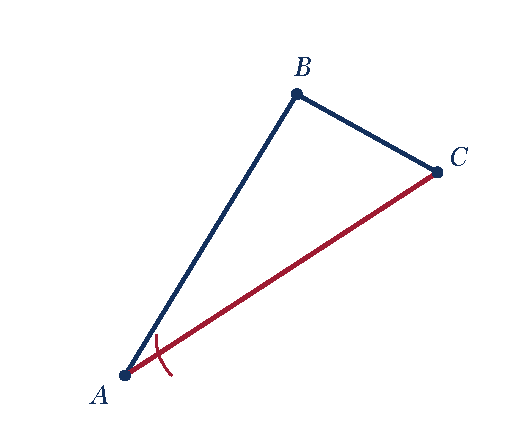
\includegraphics[width=0.75\textwidth]{figuras/pdf/cap08-fig4.pdf}
\caption{Composición de la velocidad absoluta $V'$ (dirección $AB$) y de
la velocidad de arrastre del éter (dirección $BC$): la resultante es
$AC$.}
\label{fig:cap8-4}
\end{figure}

Siendo el ángulo $A$ muy pequeño, podemos confundir su coseno con la
unidad. Despreciamos así las cantidades del orden del cuadrado de la
aberración; ahora bien, tenemos derecho a ello, pues la aberración, siendo
a lo sumo igual a $20''$ o $\tfrac{1}{10\,000}$, su cuadrado es la
$\tfrac{1}{10\,000}$-ésima parte de $20''$, es decir, $\tfrac{1}{500}$ de
segundo. Tendremos entonces
\[
AC = V' + v\Bigl(1-\frac{1}{n^2}\Bigr)\cos\varphi.
\]

Tomemos ahora ejes ligados al medio móvil. Habrá que reemplazar en la
expresión precedente la velocidad absoluta de arrastre
$v\bigl(1-\tfrac{1}{n^2}\bigr)$ por la velocidad relativa
\[
v\Bigl(1-\frac{1}{n^2}\Bigr) - v = -\frac{v}{n^2} = -v'.
\]
Por consiguiente tendremos para la velocidad de la luz respecto de estos
ejes
\[
V' - v'\cos\varphi.
\]

\section{El tiempo de recorrido en un medio en movimiento}

\noindent\textbf{237. Tiempo empleado por la luz para pasar de un punto a
otro de un medio en movimiento.} — Consideremos un rayo luminoso que va de
un punto $A_0$ a un punto $A_n$ de un medio en movimiento siguiendo la
línea quebrada $A_0A_1\ldots A_n$ (figura~\ref{fig:cap8-5}). Para pasar del
punto $A_1$ al punto $A_2$, el rayo empleará un tiempo igual a
$\dfrac{A_1A_2}{V'-v'\cos\varphi}$. Desarrollemos esta cantidad según las
potencias crecientes de $v'$, deteniéndonos en la primera potencia;
tendremos
\[
\frac{A_1A_2}{V'} + \frac{A_1A_2\cos\varphi}{V'^2}v'.
\]

\begin{figure}[h]
\centering
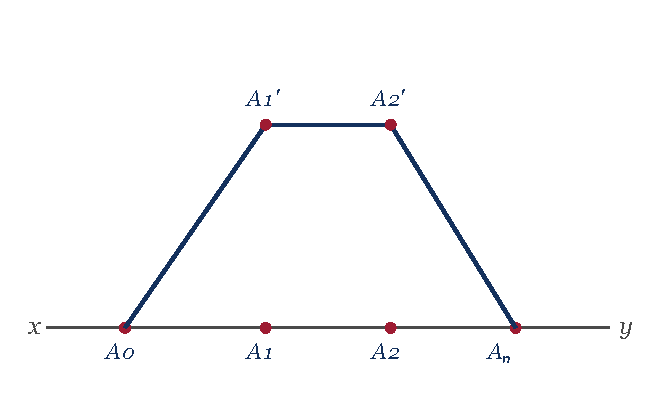
\includegraphics[width=0.85\textwidth]{figuras/pdf/cap08-fig5.pdf}
\caption{Camino en línea quebrada $A_0A_1\ldots A_n$ seguido por la luz
en un medio en movimiento.}
\label{fig:cap8-5}
\end{figure}

Si trazamos una recta $xy$ paralela a la velocidad del medio en movimiento,
el ángulo de las diversas porciones de la línea quebrada con esta recta es
precisamente el ángulo de aberración $\varphi$ que entra en la expresión
precedente; por consiguiente, $A_1A_2\cos\varphi$ es igual a la proyección
$A_1'A_2'$ de $A_1A_2$ sobre $xy$, y el tiempo empleado por la luz para ir
de $A_1$ a $A_2$ se convierte en
\[
\frac{A_1A_2}{V'} + \frac{A_1'A_2'}{V'^2}v'.
\]
Tenemos, además, $v'=\dfrac{v}{n^2}$ y $V'=\dfrac{V}{n}$, siendo $v$ la
velocidad de traslación del medio y $V$ la velocidad de la luz en el
vacío; reemplazando $v'$ y $V'$ por estos valores en la suma precedente,
tendremos
\[
\frac{A_1A_2}{V'} + A_1'A_2'\,\frac{v}{V^2}.
\]
El tiempo empleado para ir del punto $A_0$ al punto $A_n$ será la suma de
cantidades semejantes, es decir,
\[
\sum\frac{A_1A_2}{V'} + \frac{v}{V^2}A_0'A_n'.
\]
El primer término $\sum\dfrac{A_1A_2}{V'}$ representa el tiempo que
emplearía la luz si el medio estuviera en reposo; el segundo no depende más
que de la posición de los puntos extremos y de ningún modo del camino
recorrido por la luz para ir de uno al otro de esos puntos.

\section{Fenómenos ópticos en un medio en movimiento}

\noindent\textbf{238. Fenómenos ópticos en un medio en movimiento.} — Una
consecuencia importante de la fórmula precedente es que las leyes de la
reflexión y de la refracción, los fenómenos de interferencias no son
afectados por el movimiento de la Tierra.

Consideremos en particular el fenómeno de la refracción. Si $A$ y $B$
(figura~\ref{fig:cap8-6}) son dos puntos situados en dos medios diferentes,
el camino $ACB$ seguido por la luz para ir de $A$ a $B$ es tal que el
tiempo empleado para recorrer ese camino es mínimo. Para mostrar que las
leyes de la refracción son las mismas cuando los dos medios están en reposo
o en movimiento, nos basta mostrar que, si $ACB$ es el camino más corto
cuando los medios están en reposo, lo es todavía cuando los dos medios
están animados del mismo movimiento.

\begin{figure}[h]
\centering
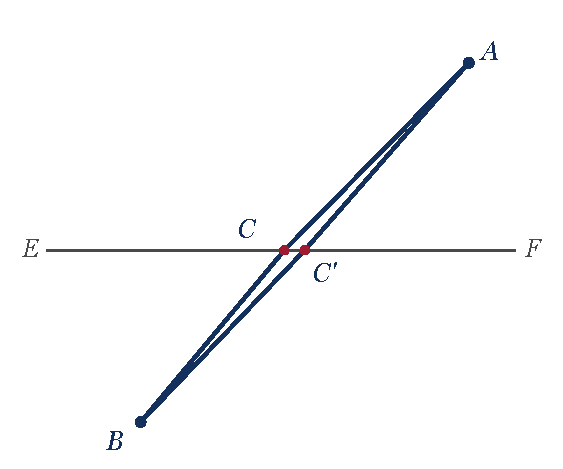
\includegraphics[width=0.6\textwidth]{figuras/pdf/cap08-fig6.pdf}
\caption{El camino mínimo $ACB$ entre dos puntos de medios distintos: su
posición no cambia cuando ambos medios se mueven con la misma
velocidad.}
\label{fig:cap8-6}
\end{figure}

Sean $T$ el tiempo empleado por la luz para ir de $A$ a $B$ por el camino
mínimo cuando los medios están en reposo; $T'$ el tiempo necesario para
recorrer un camino infinitamente vecino $AC'B$. Si $ACB$ es el que
corresponde a las leyes de la refracción, se tiene $T<T'$. Ahora bien,
según lo que acabamos de decir anteriormente, los tiempos empleados para
recorrer los caminos $ACB$ y $AC'B$ en el caso en que los medios están
animados de un movimiento de traslación cuya velocidad es $v$, son
\[
T_1 = T + \frac{v}{V^2}A'B', \qquad T_1' = T' + \frac{v}{V^2}A'B',
\]
siendo $A'B'$ la proyección de $AB$ sobre una recta paralela a la velocidad
$v$; no difieren de $T$ y de $T'$ más que por una misma cantidad. Si,
pues, se tiene $T<T'$, tendremos $T_1<T_1'$, y el camino más corto en los
medios en reposo seguirá siendo el más corto cuando los medios estén en
movimiento. Las leyes de la refracción son, por consiguiente, las mismas
en los dos casos.

Los fenómenos de interferencia de los rayos luminosos tampoco dependen del
movimiento del medio donde se producen. Si $T$ y $T'$ son los tiempos
empleados por dos rayos para ir de un punto $A_0$ a un punto $A_n$ en el
caso en que el medio está en reposo, estos tiempos serán ambos aumentados
en la misma cantidad si se supone el medio en movimiento; por consiguiente
la diferencia de los tiempos no variará y los fenómenos de interferencia
seguirán siendo los mismos en los dos casos.

En una palabra, los fenómenos ópticos no pueden poner en evidencia más que
los movimientos relativos, respecto del observador, de la fuente luminosa y
de la materia ponderable. Esto
es lo que ocurre en la aberración, donde el observador y el astro
observado no están animados del mismo movimiento; esto es también lo que
ocurre en la experiencia de Fizeau, donde el agua contenida en los tubos
posee un movimiento relativo respecto del observador. Un solo hecho no
concordaría con estas conclusiones; es la variación del plano de
polarización de la luz reflejada sobre el vidrio con la orientación de la
dirección luminosa respecto de la velocidad de rotación de la Tierra. Esta
influencia ha sido comprobada por Fizeau, pero la dificultad de las
experiencias no le ha permitido estar absolutamente seguro de ello.

\section{La hipótesis de Fresnel}

\noindent\textbf{239. Hipótesis de Fresnel.} — La explicación que hemos
dado de la aberración y las consecuencias que hemos sacado de la expresión
del tiempo empleado por la luz para ir de un punto a otro de un medio en
movimiento reposan sobre la hipótesis de que la velocidad de arrastre del
éter contenido en un medio en movimiento es
$v\bigl(1-\tfrac{1}{n^2}\bigr)$.

\begin{enunciado}{Coeficiente de arrastre de Fresnel}
La velocidad de arrastre del éter contenido en un medio material animado
de una velocidad $v$ es
\[
v\Bigl(1-\frac{1}{n^2}\Bigr),
\]
siendo $n$ el índice de refracción de la sustancia atravesada por la luz.
\end{enunciado}

El índice de refracción $n$ no es una constante; varía con el color del
rayo luminoso y no es el mismo para un rayo ordinario y un rayo
extraordinario en un medio birrefringente. Resulta de ello que la velocidad
de arrastre del éter no es la misma según se considere un rayo
extraordinario u ordinario, o bien dos rayos de colores distintos. Se ha
podido verificar, por medio de experiencias suficientemente precisas, que
el rayo ordinario y el rayo extraordinario no son arrastrados de la misma
manera. Así, pues, no debe admitirse, como parece hacerlo Fresnel, que la
velocidad de arrastre del éter es independiente de la longitud de onda de
la luz e igual al valor medio de los valores que toma para una infinidad de
valores de la longitud de onda.

Fresnel suponía que, cuando un medio transparente está en movimiento, la
masa de éter arrastrada por el movimiento era el exceso de la masa
contenida en el medio en movimiento sobre la masa que estaría contenida en
un mismo volumen del medio circundante. Llamando $\rho_0$ a la densidad del
éter en este último, $\rho$ a la densidad en el medio en movimiento,
$\rho-\rho_0$ será la densidad del éter arrastrado. Para tener la velocidad
aparente de arrastre del éter contenido en el medio en movimiento, no
tenemos más que buscar la velocidad del centro de gravedad de dos
moléculas $M$ y $M'$, de las cuales una tiene por masa $\rho_0$ y permanece
en reposo, y la otra, $M'$, tiene por masa $\rho-\rho_0$ y posee la
velocidad $v$ del medio en movimiento. Si llamamos $v_1$ a la velocidad del
centro de gravedad, tendremos, aplicando el teorema de las cantidades de
movimiento,
\[
(\rho-\rho_0+\rho_0)v_1 = (\rho-\rho_0)v + \rho_0\times 0;
\]
de donde
\[
v_1 = \frac{\rho-\rho_0}{\rho}v.
\]
Ahora bien, en la teoría de Fresnel se tiene, designando por $V_0$ y $V$
las velocidades de propagación de las ondas luminosas en los medios de
densidad $\rho_0$ y $\rho$,
\[
\frac{\rho_0}{\rho} = \frac{V^2}{V_0^2} = \frac{1}{n^2};
\]
por consiguiente tenemos para la velocidad aparente de arrastre del éter
\[
v_1 = \Bigl(1-\frac{1}{n^2}\Bigr)v.
\]
No hay ahí más que una simple visión de conjunto con la que es difícil
contentarse, pero vamos a buscar justificar el modo de ver de Fresnel
mediante un análisis más riguroso.

\section{Velocidad de propagación en un medio en movimiento}

\noindent\textbf{240. Velocidad de propagación en un medio en movimiento.}
— Podemos darnos cuenta del arrastre aparente del éter estudiando la
propagación de una onda plana en un medio en movimiento y admitiendo que el
desplazamiento de las moléculas de éter depende del desplazamiento de las
moléculas materiales. Si designamos por $\xi$ y $\xi_1$ las componentes
según el eje de las $x$ de los desplazamientos de las moléculas de éter y
de materia, tendremos, en el caso en que el medio material no esté animado
de un movimiento de traslación, las siguientes ecuaciones (\S 142 del
Capítulo V):\footnote{Aquí Poincaré reinicia la numeración de ecuaciones
del capítulo, como ya ha ocurrido en capítulos anteriores. Se conserva la
numeración de Poincaré.}
\setcounter{equation}{0}
\begin{align}
\rho\,\frac{d^2\xi}{dt^2} &= \Delta\xi - \frac{d\Theta}{dx} + M(\xi_1-\xi). \\
\rho_1\,\frac{d^2\xi_1}{dt^2} &= M(\xi-\xi_1).
\end{align}

Supongamos ahora que, permaneciendo el éter en reposo, el medio material
posee un movimiento de traslación de velocidad $v$ normal al plano de la
onda; tomemos para plano de las $yx$ un plano paralelo al plano de la onda
y busquemos qué se convierten las ecuaciones precedentes.

$\xi_1$ es una función de $z$ y de $t$ solamente. Cuando el medio está en
reposo, la velocidad de la molécula material en el instante $t$ es
$d\xi_1/dt$; pero, a causa del movimiento de traslación que posee este
medio, la $z$ de la posición de equilibrio de la molécula aumenta en
$v\,dt$ durante el tiempo $dt$. Por consiguiente, el incremento de $\xi_1$
para un incremento $dt$ del tiempo será\footnote{La fe de erratas del
propio volumen original señala que la edición impresa de 1889 trae aquí,
en la página 394, línea 12, el error tipográfico $d\xi_1/d\xi$ en el primer
término (con $\xi$ en el denominador en vez de $t$), y pide leer
$d\xi_1/dt$. La forma que se da aquí ya es la corregida.}
\[
\frac{d\xi_1}{dt}dt + \frac{d\xi_1}{dz}dz = \frac{d\xi_1}{dt}dt +
\frac{d\xi_1}{dz}v\,dt,
\]
y la velocidad de la molécula material en el instante $t$ tendrá por valor
\[
w = \frac{d\xi_1}{dt} + \frac{d\xi_1}{dz}v.
\]
La aceleración en este mismo instante será\footnote{El original imprime
en el último término de la fórmula siguiente
$\frac{dw}{dt}\frac{dz}{dt}$; se lee $\frac{dw}{dz}\frac{dz}{dt}$, que es
lo que exige la regla de derivación y lo que da el resultado que sigue.
Esta segunda errata, a pocas líneas de la anterior, no figura en la fe de
erratas del volumen.}
\[
\frac{dw}{dt} = \frac{dw}{dt} + \frac{dw}{dz}\frac{dz}{dt},
\]
estando las derivadas de $w$, puestas en el segundo miembro, tomadas como
derivadas parciales. Reemplazando en esta expresión $w$ por su valor,
tenemos para la aceleración
\[
\frac{d^2\xi_1}{dt^2} + 2v\frac{d^2\xi_1}{dz\,dt} +
v^2\frac{d^2\xi_1}{dz^2}.
\]
La ecuación del movimiento de la molécula material es, pues, despreciando
el cuadrado de $v$,
\begin{equation}
\rho_1\Bigl(\frac{d^2\xi_1}{dt^2} + 2v\frac{d^2\xi_1}{dz\,dt}\Bigr) =
M(\xi-\xi_1).
\end{equation}
Tal es la ecuación que debe reemplazar a la ecuación (2). En cuanto a la
ecuación (1), se reduce, en el sistema de ejes adoptado, a
\begin{equation}
\rho\,\frac{d^2\xi}{dt^2} = \frac{d^2\xi}{dz^2} + M(\xi_1-\xi),
\end{equation}
puesto que $\xi$ ya no depende más que de $z$ y de $t$.

La suma de estas dos últimas ecuaciones elimina $M$ y nos da
\begin{equation}
\rho\,\frac{d^2\xi}{dt^2} + \rho_1\Bigl(\frac{d^2\xi_1}{dt^2} +
2v\frac{d^2\xi_1}{dz\,dt}\Bigr) = \frac{d^2\xi}{dz^2}.
\end{equation}
Supondremos que $M$ es muy grande; la ecuación (4) muestra entonces que
$M(\xi_1-\xi)$ es finito. Se concluye de ello que $\xi_1-\xi$ es muy pequeño
y nos vemos llevados a admitir, a título de primera aproximación, que se
tiene $\xi=\xi_1$. La ecuación (5) se convierte entonces en
\begin{equation}
(\rho+\rho_1)\frac{d^2\xi}{dt^2} + 2v\rho_1\frac{d^2\xi}{dz\,dt} =
\frac{d^2\xi}{dz^2}.
\end{equation}
La ecuación del movimiento en el vacío se deducirá de la precedente
haciendo en ella $\rho_1=0$; sabemos que, en este caso, la velocidad de
propagación es
\[
V = \frac{1}{\sqrt{\rho}}.
\]
Si suponemos el movimiento luminoso propagándose en un medio material en
reposo, hay que hacer $v=0$ en la ecuación (6), que da entonces para la
velocidad de propagación
\[
\frac{1}{\sqrt{\rho+\rho_1}}.
\]
Por consiguiente, el índice de refracción de la sustancia es
\[
n = \sqrt{\frac{\rho+\rho_1}{\rho}}.
\]

Para tener la velocidad de propagación en el caso en que el medio material
esté animado de un movimiento de traslación según el eje de las $z$,
busquemos satisfacer la ecuación (6) con el siguiente valor de $\xi$,
\[
\xi = e^{\frac{2i\pi}{\lambda}(z-Vt)}.
\]
Obtendremos, tras suprimir los factores comunes a los dos miembros,
\[
(\rho+\rho_1)V^2 - 2vV\rho_1 = 1;
\]
de donde sacamos
\[
V^2 = \frac{1}{\rho+\rho_1} + \frac{2vV\rho_1}{\rho+\rho_1}.
\]
Difiriendo poco este valor $V$ de la velocidad de propagación en el mismo
medio supuesto inmóvil, podemos, en el segundo miembro de la igualdad
precedente, reemplazar $V$ por su valor aproximado
$\tfrac{1}{\sqrt{\rho+\rho_1}}$, y tenemos
\[
V^2 = \frac{1}{\rho+\rho_1} + \frac{2v\rho_1}{(\rho_1+\rho)\sqrt{\rho+\rho_1}},
\]
o, puesto que hemos despreciado las cantidades que contenían el cuadrado de
$v$,
\[
V = \frac{1}{\sqrt{\rho+\rho_1}} + \frac{v\rho_1}{\rho+\rho_1}.
\]
Todo sucede, pues, como si el éter se encontrara arrastrado con una
velocidad igual a
\[
\frac{v\rho_1}{\rho+\rho_1}.
\]
Esta fórmula puede, por lo demás, escribirse
\[
v\Bigl(1-\frac{\rho}{\rho+\rho_1}\Bigr),
\]
o, puesto que $n=\sqrt{\tfrac{\rho+\rho_1}{\rho}}$,
\[
v\Bigl(1-\frac{1}{n^2}\Bigr).
\]
Volvemos a encontrar, pues, la misma expresión que en las teorías de
Fresnel. No es esto más que una primera aproximación. En efecto, $\xi_1-\xi$
no es nulo, sino solamente muy pequeño; la diferencia es del orden de la
dispersión.

El análisis del n.\textsuperscript{o}~142 muestra que la razón
$\xi_1/\xi$, que es vecina de la unidad, depende de la longitud de onda.
Para dar cuenta de las experiencias que, como hemos visto, dan para la
velocidad de arrastre $v\bigl(1-\tfrac{1}{n^2}\bigr)$, \emph{siendo $n$ el
índice de refracción del color considerado}, hay que admitir que esta razón
es, \emph{cualquiera que sea el color}, independiente de $v$; no conocemos ninguna
teoría satisfactoria que justifique esta hipótesis.
